% 03.3. INFORMACIÓN DE DISEÑO DE COMPONENTES RELEVANTES DEL SISTEMA
%----------------------------------------------------------------------------------------------
\vspace{.2cm}
\begin{figure}[ht]
\centerline{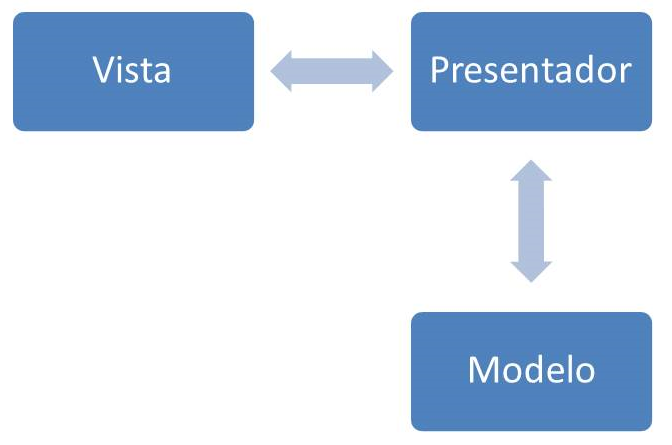
\includegraphics[scale=0.6]{img/componentes}}\
\caption{Componentes relevantes del sistema}
\label{fig:diagCompon}
\end{figure}

Los componentes relevantes del sistema son los que ya han sido explicados en el apartado de Aspectos Arquitecturales y Tecnológicos, propios del patrón de diseño de Modelo-Vista-Presentador. Hemos elegido este patrón de diseño porque consideramos que es un patrón que se ajusta perfectamente al problema que tenemos que resolver y a su vez ofrece una solución lo más sencilla posible.